\documentclass[fleqn]{report}
\usepackage{fullpage}
\usepackage{titlesec}
\usepackage{amsmath}
\usepackage{mathtools}
\usepackage{graphicx}
\usepackage{hyperref}
\usepackage{caption}
\usepackage{subcaption}
\graphicspath{ {./figs/} }
\DeclareUnicodeCharacter{2212}{-}
\titleformat{\chapter}[display]{\normalfont\bfseries}{}{0pt}{\Huge}
\renewcommand{\baselinestretch}{2}
\providecommand{\abs}[1]{\left\vert#1\right\vert}

\begin{document}
	\begin{titlepage}
		\begin{center}
			\vspace*{1cm}
			\textbf{\Huge Magnetic field line Diffusion in Plasma Reconnection}{\Huge}\\
			\text{\large Project Report}\\
			\vspace{1.5cm}
			\textbf{\Large Devananth V}\\
			\text{EP20BTECH11004}\\
			\vspace{1cm}
			\textbf{\LARGE Engineering Physics,\\ Department of Physics}\\
			\vspace{1cm}
			
			\begin{figure}[!h]
				\centering
				
\includegraphics[scale=0.1]{/iith.png}	
			\end{figure}	
			\vspace{1cm}
			\text{\Large Supervisor: Kirit Kumar Makwana}\\
			\text{\large April 2023}\\
		\end{center}
	\end{titlepage}
	\tableofcontents
	\begin{abstract}
	This is the report on the project "Magnetic field line diffusion in plasma reconnection", conducted from August 2022 to April 2023 under the guidance of Assistant Professor Kirit Kumar Makwana.\\
	Magnetic field lines are continuously created and destroyed inside a turbulent plasma due to magnetic reconnection. In such a turbulent system, the particles are chaotic and diffuse. We try to find what happens to magnetic field lines in such a plasma system. If they do diffuse, we also try to find the nature of this diffusion.\\
	We use Python code to plot magnetic field lines from simulated magnetic field vector data. We then observe the field lines by plotting them. We also look at field lines passing through a local initial point and how they disperse with distance from the initial point. 
		
	\end{abstract}
	\chapter{Introduction}
	\section{Magnetic Field Lines in Plasma}
	Plasma is one of the four states of matter made up of ions. Magnetohydrodynamics(MHD) treats the plasma as a single fluid governed by a combination of Maxwell's equations and the Navier–Stokes equations.\\
	Plasma turbulence produces a tangled magnetic field on its own. If the magnetic field contains much energy, an instability might generate plasma flow, causing the field to reorganize. This phenomenon is called Magnetic Reconnection. In dynamic plasmas, the energy conversion between the magnetic field and the plasma flow happens constantly. The plasma's magnetic structures strongly influence the conversion's amount and direction. In resistive MHD, turbulence has also shown to accelerate reconnection.\\
	\begin{figure}[!h]
		\centering
		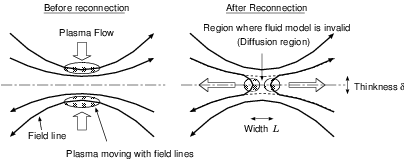
\includegraphics[scale=0.8]{/reconnection.png}
		\caption{Magnetic Reconnection in Plasma}
		\label{fig:recon}
	\end{figure}\\
	 In the diffusion region where the magnetic field is inhomogeneous, the sporadic energy released through magnetic reconnection make field lines chaotic.
	\begin{figure}[!ht]
		\centering
		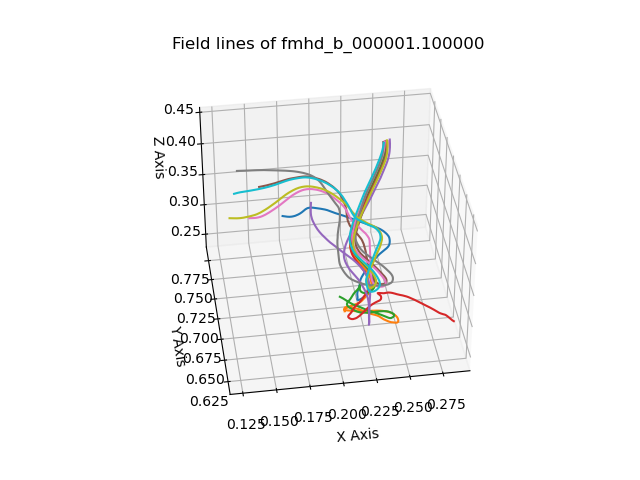
\includegraphics[scale=0.7]{/chaos.png}
		\caption{Chaotic Field Lines}{The Field lines are seen to diffuse}
		\label{fig:chaos}
	\end{figure}
	\section{Diffusion and Types}
	 Diffusion is the net movement of anything generally from a region of higher concentration to a region of lower concentration. Diffusion is driven by a gradient in Gibbs free energy or chemical potential. A distinguishing feature of diffusion is that it depends on particle random walk, and that it results in mixing or mass transport without requiring the directed bulk motion.
	 \subsection{Normal Diffusion}
	  In a typical diffusion process, like Brownian motion, described by Einstein and Smoluchowski, the Mean Square Distance(MSD) is linear in time. It is shown by the blue line in the figure below. $[r^{2} \propto t]$\\
	  \begin{figure}[!ht]
	  	\centering
	  	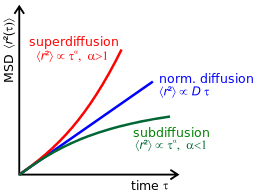
\includegraphics[scale=0.7]{/diffusion.png}
	  	\caption{Types of Diffusion}
	  	\label{fig:diff}
	  \end{figure}
  	\subsection{Anomalous diffusion}
  	 Anomalous diffusion is a diffusion process with a non-linear relationship between the mean squared displacement (MSD) and time. Consider $r^{2} \propto t^ \alpha$ where $\alpha !=1$.\\
  	 \textbf{Subdiffusion:} Subdiffusion is shown by the green curve, where we can see that $r^{2} \propto t^{\alpha}$ where $\alpha < 1$\\
  	 \textbf{Superdiffusion:} Superdiffusion is shown by the red curve, where we can see that $r^{2} \propto t^{\alpha}$ where $\alpha > 1$\\
  	 \textbf{Richardson Diffusion:} The Richardson diffusion describes the explosive growth of the separation of particles in a turbulent medium. It is inferred from previous fluids experiments. It is a type of superdiffusion with $\alpha\sim 3$. 
  	 \subsection{Changes Made}
  	 In this project, we are taking "l", where "l" is the distance traveled from the initial point, as analogous to "t" given above.\\ Also, in this report, we are taking diffusion in terms of "r" and not "$r^{2}$", by which $\alpha$ becomes $\frac{\alpha}{2}$.  
	\chapter{Methodology - Python Code}
	\section{Magnetic Field Lines}
	\subsection{Field Line Equation}
	We know that the field line is tangential to the field vector. Here, $\vec{B}$ is the field vector, $\vec{dr}$ is the differential element for the position vector, and $\vec{dl}$ is the field line differential.
		\begin{align}
		\hat{b}=\frac{\vec{B}}{\abs{B}}\\
		\vec{dr}=\hat{b}dl\\
		dx\hat{i}+dy\hat{j}+dz\hat{k}=b_{x}dl\hat{i}+b_{y}\hat{j}+b_{z}dl\hat{k}
	\end{align}
	Equating the coefficients, we get 3 Ordinary Differential Equation(ODE):
	\begin{align}
		\frac{dx}{dl}=b_{x}=\frac{B_{x}(x,y,z)}{\abs{B}}\\
		\frac{dy}{dl}=b_{y}=\frac{B_{y}(x,y,z)}{\abs{B}}\\
		\frac{dz}{dl}=b_{z}=\frac{B_{z}(x,y,z)}{\abs{B}}
	\end{align} 
	By solving the given ODEs we get x=x(l), y=y(l), and z=z(l), using which we can trace field lines for different values of 'l'. 
	\subsection{Runge-Kutta Method}
	We use the 4th Order Multivariable Adaptive Step-size Runge-Kutta Method, to solve the ODEs. In fourth order Runge-Kutta, we use the equation given below to integrate the ODEs.
	\begin{align}
		k_{1}=hf(x_{n},y_{n}),\\
		k_{2}=hf(x_{n}+\frac{h}{2}, y_{n}+\frac{k_{1}}{2}),\\
		k_{3}=hf(x_{n}+\frac{h}{2}, y_{n}+\frac{k_{2}}{2}),\\
		k_{4}=hf(x_{n}+h, y_{n}+k_{3}),\\
		y_{n+1}=y_{n}+\frac{k_{1}}{6}+\frac{k_{2}}{3}+\frac{k_{3}}{3}+\frac{k_{4}}{6}+O(h^{5}).
	\end{align}
	In the said method the step-size is varied on the situation to decrease computation time and  increase accuracy. We decrease the step-size when the error is above desired error. Otherwise we increase the step-size. It is made multivariable by considering the variables as vectors. 
	\subsection{Trilinear Interpolation}
	To use the Runge-Kutta method we require continuous values, however, our data is discrete. To solve this, we use Trilinear Interpolation(3D-Interpolation) to get the required points. Trilinear Interpolation is the process of linearly interpolating points within a box (3D) with values given at the box’s vertices. Trilinear interpolation is implemented by taking linear interpolation of two bilinear interpolations.
		\begin{figure}[!ht]
		\centering
		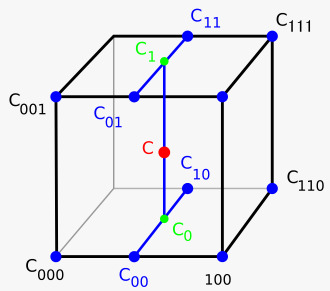
\includegraphics[scale=0.4]{/inter.png}
		\caption{$c_{000},c_{100}$... etc.,are the known values, which is used to form the corner points of the 3D box.}
		\label{fig:inter}
	\end{figure}
	\section{Diffusion of Magnetic Field Lines}
	We use the magnetic field line data from above to find the diffusion of magnetic field lines. For this we consider magnetic field lines originating from the same locality and measure the mean distance between the field lines for each value of "l". Here, we run into a problem. In our data, the values of "l" may be different for each field line. This is because we are using variable step-size in the Runge-Kutta method. To overcome this, we use the \textbf{interp()} function available in the NumPy library.\\
	The interp(x,xp,yp) function returns the corresponding values of y(within yp) for the given x(within xp). 
	\begin{figure}[!ht]
		\centering
		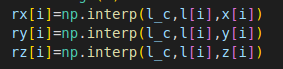
\includegraphics[scale=0.7]{/interp.png}
		\caption{1-D Interpolation Function}
		\label{fig:interp}
	\end{figure}\\
	To find the diffusion of magnetic field lines in the plasma, we take 'n' different localities with 'm' magnetic field lines each. For each value of "l", we find the mean distance between the 'm' field lines for the 'n' points and take their average. We do this to get an accurate representation of the diffusion of the plasma.\\ 
	The code snippet is given below.
	\begin{figure}[!ht]
		\centering
		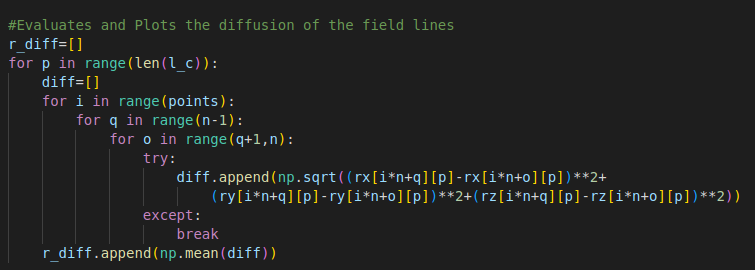
\includegraphics[scale=0.5]{/diff.png}
		\caption{Evaluating Diffusion}
		\label{fig:dif}
	\end{figure}\\ 	
	\chapter{Observations}
	\section{Magnetic Field lines}
	\subsection{Field lines at a Seperation}
	The images given below show the form of the field lines at 't=0' and 't=100000' with initial points in a straight line parrallel to z-axis(x=0.2 and y= 0.7) at a seperation.
	\begin{figure}[!ht]
		\centering
		\begin{subfigure}{.5\textwidth}
			\centering
			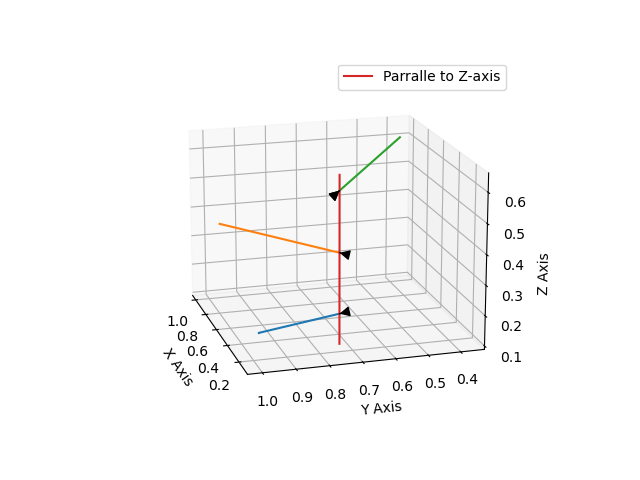
\includegraphics[scale=0.5]{/tz0.png}
		\caption{Field lines at T=0}
		\label{fig:tz0}
	\end{subfigure}%
	\begin{subfigure}{.5\textwidth}
		\centering
		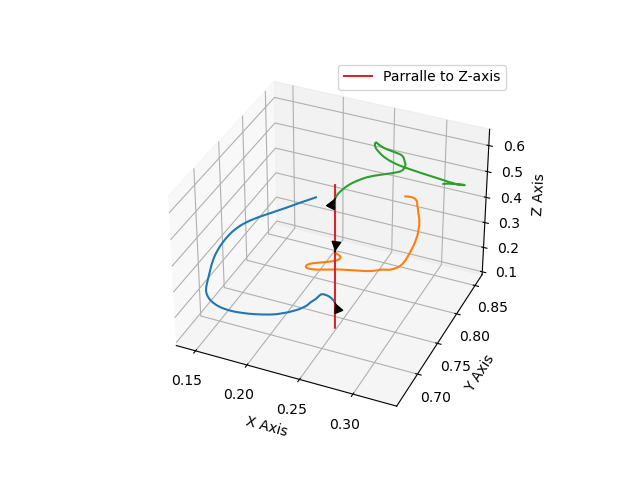
\includegraphics[scale=0.5]{/tz10.png}
		\caption{Field Lines at T=100000}
		\label{fig:tz10}
	\end{subfigure}
	\caption{Field lines around a straight line parrallel to z-axis}
	\label{fig:tz}
	\end{figure}\\\\
	We observe parrallel field lines at 't=0' which becomes chaotic at 't=100000', due to plasma turbulance.
	The field lines at 't=0' are straight lines rotated spherically about the line parrallel to the z-axis as the magnetic field is of a current sheet. However, at 't=100000', it loses its shape due to turbulence.\\ 
	\subsection{Adjoining Field Lines}
	The images given below show the form of the field lines at 't=0' and 't=100000' with adjoined initial points.
	\begin{figure}[!ht]
		\centering
		\begin{subfigure}{.5\textwidth}
			\centering
			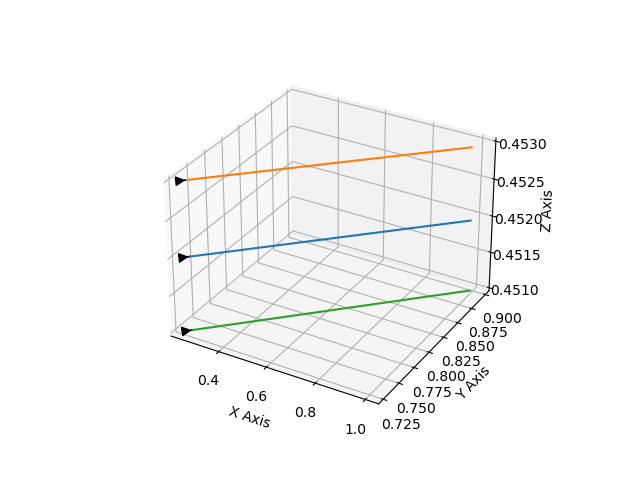
\includegraphics[scale=0.5]{/t0.png}
			\caption{Field lines at T=0}
			\label{fig:sub1}
		\end{subfigure}%
		\begin{subfigure}{.5\textwidth}
			\centering
			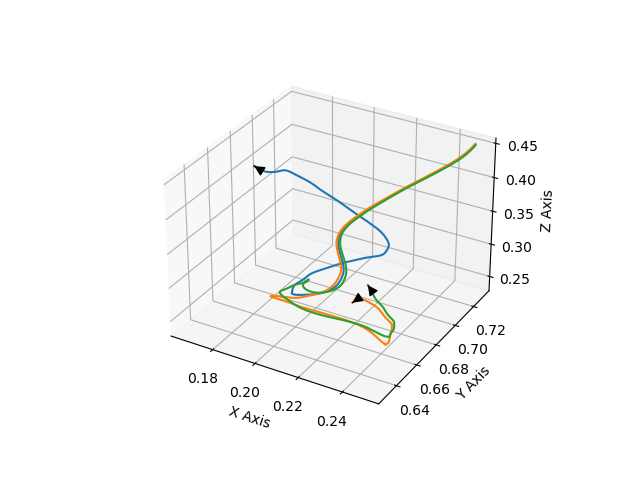
\includegraphics[scale=0.5]{/t10.png}
			\caption{Field Lines at T=100000}
			\label{fig:sub2}
		\end{subfigure}
		\caption{Field lines with initial points close to each other}
		\label{fig:test}
	\end{figure} \\
	We observe parallel field lines at 't=0', which becomes chaotic at 't=100000'. In Figure(a), we observe that field lines close to each other form straight parallel lines, when there is no turbulence(t=0). However, at 't=100000', we observe that the field lines diffuse chaotically due to turbulence. We can observe that the field lines travels without dispersing much initially but then disperses rapidly.\
	\section{Diffusion of Field Lines}
	To find the mean diffusion of magnetic field line in the plasma we take 3 diffrent localities with 10 magnetic field lines each. The below given image shows the plot of "log(Diffusion)" vs "log(l)".
	\begin{figure}[!ht]
		\centering
		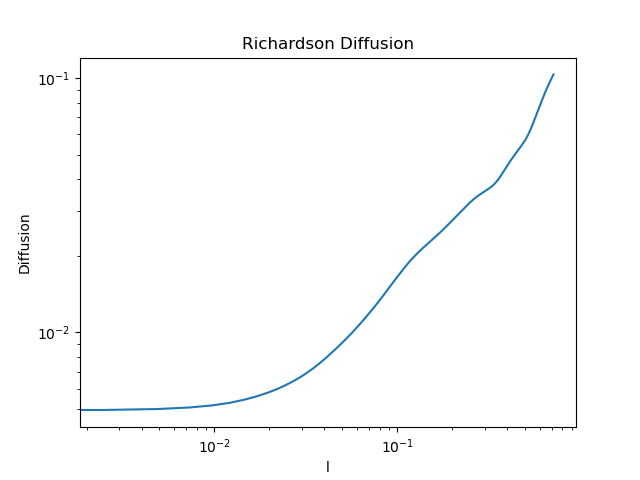
\includegraphics[scale=0.7]{/plot.png}
		\caption{Plot of diffusion vs "l"}
		\label{fig:plot}
	\end{figure}\\
	The graph shows that diffusion initially does not change much with 'l', however, after some distance the plot becomes almost a straight line with a positive slope $\alpha$.\\
	We can try to find the slope $\alpha$ of this line.\\
	The straight line is of the form $log(r)=\alpha log(l) + c$, where $\alpha$ is the slope and c is the y-intercept. We consider two end points $(x_{1},y_{1})$ and $(x_{2},y_{2})$. 
	\begin{align}
		log(y_{1})=\alpha log(x_{1}) + c \label{eq:1}\\
		log(y_{2})=\alpha log(x_{2}) + c \label{eq:2}
	\end{align}
	Taking Eqn \eqref{eq:2} - Eqn \eqref{eq:1} we get:\\
	\begin{align}
		log(\frac{y_{2}}{y_{1}})=\alpha log(\frac{x_{2}}{x_{1}}) \\
		\alpha=\frac{log(\frac{y_{2}}{y_{1}})}{log(\frac{x_{2}}{x_{1}})}
	\end{align}\\
	We take ($x_{1}$=0.0494441, $y_{1}$=0.00927756) and ($x_{2}$=0.200011, $y_{2}$=0.351961) from the plot to calculate $\alpha$.\\
	Calculating we get \textbf{$\alpha$= 0.954066858}\\ 
	Since we get $\alpha > \frac{1}{2}$, it means that the field lines show \textbf{Superdiffusion}.
	\section{Results and Discussion}
	 Slope/Power \textbf{$\alpha$= 0.954066858}\\
	 Diffusion $r\propto l^{0.954066858}$\\
	 The Magnetic Field lines show \textbf{Superdiffusion}.\\
	 The required alpha value of 1.5 for diffusion was not achieved due to the dataset's restriction to only the earlier stages of the phenomenon under study.
	 To ensure accurate analyses, it is necessary to apply the code to a dataset that includes later stages of the phenomenon.	
	\chapter{Appendix}
	\section{Code to Plot 3D Field lines with Directional Arrows} 
	\begin{figure}[!ht]
		\centering
		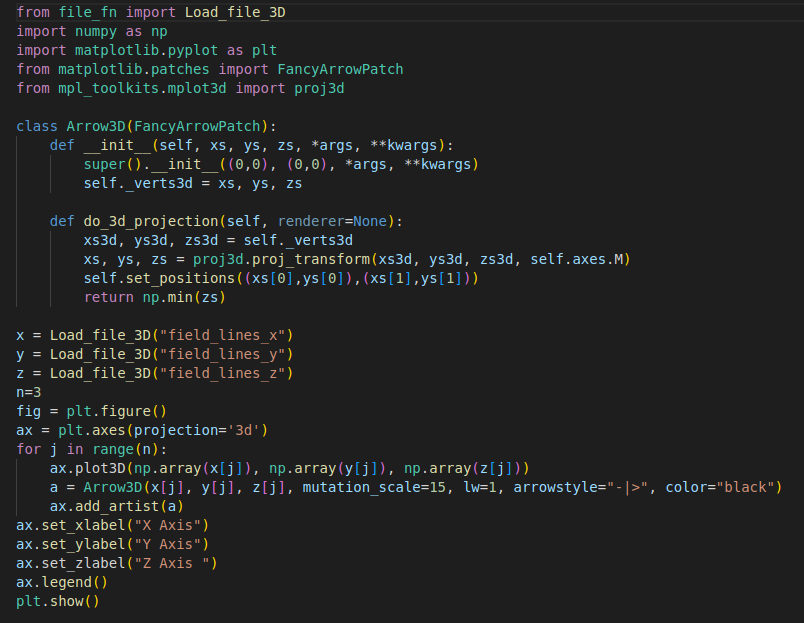
\includegraphics[scale=0.5]{/arrows.png}
		\caption{Arrows are drawn in the 3D field line using the first and second point of the field line as reference}
		\label{fig:arrows}
	\end{figure}
	\section{Change in Field Lines with 't'}
	\begin{figure}[!ht]
		\centering
		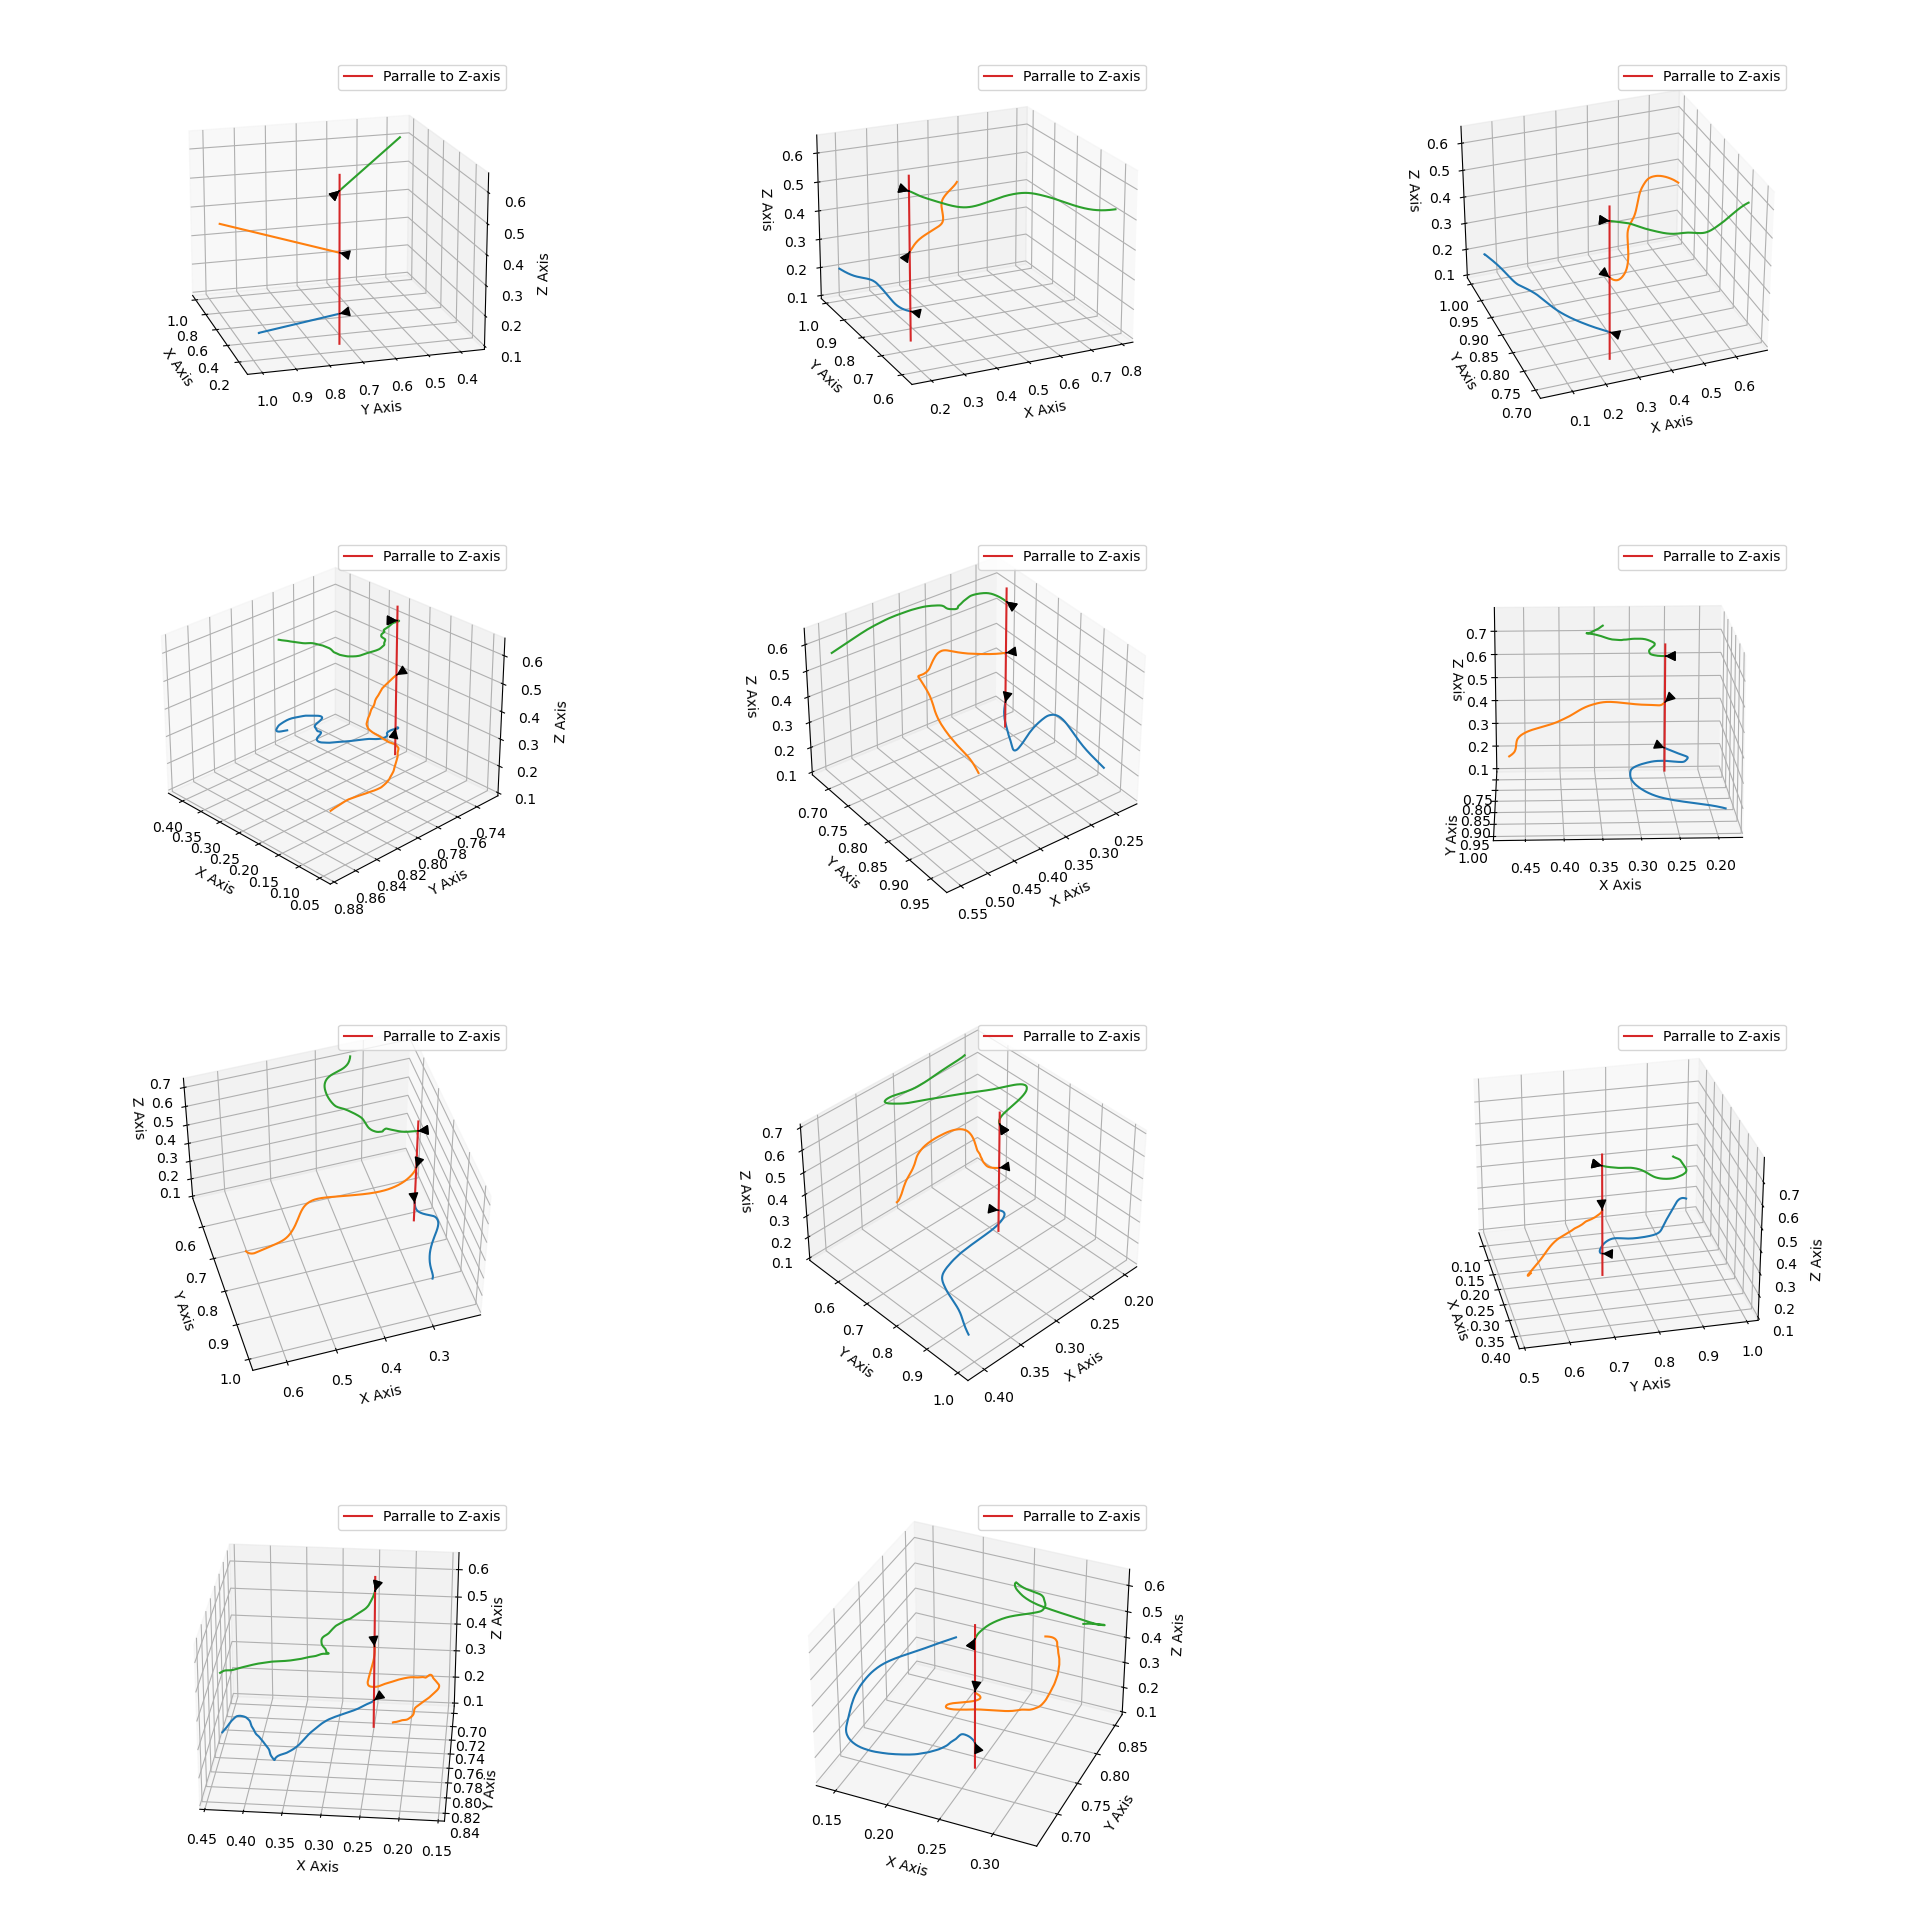
\includegraphics[scale=0.25]{/tz.png}
		\caption{'t' increases from right to left and then down}
		\label{fig:t}
	\end{figure}
	\section{Plot of Magnetic Field Lines Used in Finding Diffusion}
	\begin{figure}[!ht]
		\centering
		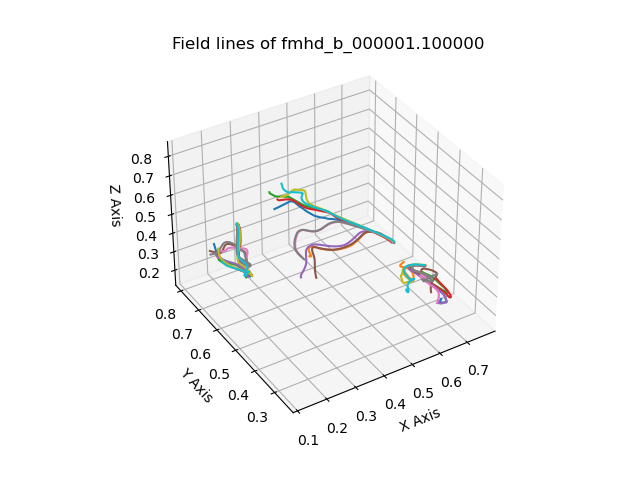
\includegraphics[scale=0.7]{/3points.png}
		\caption{Shows the 3 initial points with 10 field lines each.}
		\label{fig:3points}
	\end{figure}
	\section{Acknowledgement}
	I am incredibly grateful to Asst Prof. Kirit Kumar Makwana for providing me with an opportunity of working on this project and guiding me through it. I want to thank him for his unwavering support and patience throughout the project and his willingness to answer my numerous questions and provide timely feedback. This endeavor has taught me a lot and is an invaluable asset for my future.	
	\chapter{References}
	1. William H. Press, Saul A. Teukolsky, "Adaptive Stepsize Runge-Kutta Integration", Published by the American Institute of Physics in 1992.\\  
	2. Snehanshu Maiti, Kirit D. Makwana, Heshou Zhang, and Huirong Yan, "Cosmic-ray Transport in Magnetohydrodynamic Turbulence", Published in the The Astrophysical Journal by the American Astronomical Society on February 2022.\\
	3. Peera Pongkitiwanichakul, Kirit D. Makwana, and David Ruffolo, "Driving reconnection in sheared magnetic configurations with forced fluctuations", Published in Physics of Plasmas on February 2018.\\
	4. Abhinav Poddar, Engineering Physics, Department of Physics, Indian Institute of Technology Hyderabad, "Tracing of field lines from MHD dataset", April 2022.\\
	5. Fig: \ref{fig:recon}:"https://www.quora.com/What-are-the-necessary-conditions-for-magnetic-reconnection"\\
	6. Fig: \ref{fig:diff}: https://en.wikipedia.org/wiki/Anomalous$\_$diffusion\\
	7. Fig: \ref{fig:inter}: https://en.wikipedia.org/wiki/Trilinear$\_$interpolation\\
	7. "https://en.wikipedia.org/wiki/Magnetic$\_$reconnection","https://en.wikipedia.org/wiki/Plasma$\_$(physics)"\\
	8. "https://royalsocietypublishing.org/doi/10.1098/rsta.2014.0144"\\
	9. "https://numpy.org/doc/stable/reference/generated/numpy.interp.html"\\
	10."https://www.nature.com/articles/nature10827.pdf?pdf=reference"\\
	11."https://link.springer.com/article/10.1007/s41116-022-00032-9"\\
	12."https://www.compadre.org/nexusph/course/Diffusion$\_$and$\_$random$\_$walks"
	
\end{document}